\projectstart{c1}{C1}{Lectura del teclat}

\section{Objectius}

En aquesta pràctica es preten explicar el funcionament del teclat matricial de
la placa, les seves limitacions, i la interacció tant per polling com per interrupció.

\section{Desenvolupament}


\subsection{Descripció del teclat i procediment de lectura}

Aquest apartat és purament explicatiu, s'exposa en primer lloc l'interconnexió interna
del teclat, la connexió amb la placa, la motivació per fer el teclat matricial en comptes
de fer servir una línia GPIO per cada tecla, i la necessitat de fer una exploració
per saber quina (o quines) tecles s'han premut.

Llavors es detalla el procediment per explorar el teclat cercant una única tecla,
i la configuració que han de tenir les línies del teclat.

També s'explica com detectar dues tecles, i tres tecles o més, i el fet que, depenent
de les tecles premudes, es poden detectar «pulsacions falses» a causa de la connexió matricial.


\subsection{Codi d'exploració del teclat}

Ara implementarem el codi d'inicialització i exploració del teclat.
Es demana en primer lloc que generem els fitxers \filename{keyboard.c} i \filename{keyboard.h}
seguint l'estructura de les pràctiques anteriors, i afegim el primer al \filename{Makefile}.
Aquests canvis conformen el \commit{b66f15b0b4244b2782ead4f68a96218cee1b3724}.

\voluntari
Abans de començar la implementació, per simplificar el codi farem mètodes utilitat
per posar una línia GPIO en mode entrada (\fname{GPIO_ModeInput}), i en sortida amb
drenador obert (\fname{GPIO_ModeOpenDrain}):

\begin{minted}{c}
// Configure a GPIO line as open drain output, at the lowest speed,
// and write a high value (open state)
//     port: GPIO port
//     line: GPIO line to set as output
void GPIO_ModeOpenDrain(GPIO_TypeDef *port, int32_t line) {
    // MODERy[1:0] -> 01 General purpose output mode
    port->MODER = (port->MODER & ~(0b11 << line * 2)) | (0b01 << line * 2);

    // OTy -> 1 Open drain output
    port->OTYPER = (port->OTYPER & ~(0b1 << line)) | (0b1 << line);

    // OSPEEDRy[1:0] -> 00 Speed 25MHz
    port->OSPEEDR = (port->OSPEEDR & ~(0b11 << line * 2)) | (0b00 << line * 2);

    // PUPDRy[1:0] -> 00 No pull-up, no pull-down
    port->PUPDR = (port->PUPDR & ~(0b11 << line * 2)) | (0b00 << line * 2);

    // ODRy -> 1 Open
    port->ODR = (port->ODR & ~(0b1 << line)) | (0b1 << line);
}

// Configure a GPIO line as input
//     port: GPIO port
//     line: GPIO line to set as output
//     pullUpDown: 0 to disable pull-up / pull-down, 1 to enable pull-up
//                 resistor, 2 to enable pull-down resistor
void GPIO_ModeInput(GPIO_TypeDef *port, int32_t line, int32_t pullUpDown) {
    // MODERy[1:0] -> 00 Input
    port->MODER = (port->MODER & ~(0b11 << line * 2)) | (0b00 << line * 2);

    // PUPDRy[1:0] -> 00 No pull-up, no pull-down
    port->PUPDR = (port->PUPDR & ~(0b11 << line * 2)) | ((pullUpDown & 0b11) << line * 2);

    // ODRy -> 1
    port->ODR = (port->ODR & ~(0b1 << line)) | (0b1 << line);
}
\end{minted}
\vskip -1em

Els mètodes es defineixen a \filename{util.c}, es declaren els prototips a \filename{util.h}
i això conforma el \commit{f3cd0427d6c2123b688dfd463fa06a6c8eac80b5}.

Seguint amb la pràctica hem d'implementar (estudi previ) el mètode \fname{initKeyboard}:

%previ
\begin{minted}{c}
// Initialize the keyboard GPIO pins and resources
void initKeyboard(void) {
    // Put rows in open drain mode
    GPIO_ModeOpenDrain(KEY_PORT, KEY_ROW1_PAD);
    GPIO_ModeOpenDrain(KEY_PORT, KEY_ROW2_PAD);
    GPIO_ModeOpenDrain(KEY_PORT, KEY_ROW3_PAD);
    GPIO_ModeOpenDrain(KEY_PORT, KEY_ROW4_PAD);

    // Put columns in pull-up input mode
    GPIO_ModeInput(KEY_PORT, KEY_COL1_PAD, 1);
    GPIO_ModeInput(KEY_PORT, KEY_COL2_PAD, 1);
    GPIO_ModeInput(KEY_PORT, KEY_COL3_PAD, 1);
    GPIO_ModeInput(KEY_PORT, KEY_COL4_PAD, 1);
}
\end{minted}
\vskip -1em
%/previ

S'emplena el codi a \filename{keyboard.c}, es defineix el prototip de la funció a
\filename{keyboard.h}, es documenta adequadament, i es crida des de \fname{main}.

Ara es demana fer una funció \mintinline{c}|int32_t readKeyboard(void)| que faci
una exploració del teclat i retorni un codi identificant la tecla premuda.
Si no s'ha detectat cap tecla preumda, es retornarà un codi especial.

Els codis s'assignaran com es detalla a continuació:

\begin{multicols}{2}
\centering

\begin{tabular}{cc}
\toprule
Codi & Tecla \\ \midrule
0 & \texttt{1} \\
1 & \texttt{2} \\
2 & \texttt{3} \\
3 & \texttt{A} \\
4 & \texttt{4} \\
5 & \texttt{5} \\
6 & \texttt{6} \\
7 & \texttt{B} \\
\bottomrule
\end{tabular}

\begin{tabular}{cc}
\toprule
Codi & Tecla \\ \midrule
8 & \texttt{7} \\
9 & \texttt{8} \\
10 & \texttt{9} \\
11 & \texttt{C} \\
12 & \texttt{*} \\
13 & \texttt{0} \\
14 & \texttt{\#} \\
15 & \texttt{D} \\
32 & (cap) \\
\bottomrule
\end{tabular}

\end{multicols}

Un avantatge d'aquest codi és que els dos bits més alts corresponen a la fila
de la tecla i els dos bits més baixos, a la columna.

\voluntari
Per mantenir el codi net i permetre canviar l'assignació de codis en el futur (si
canviessim de teclat, per exemple) sense haver de canviar tot el codi que fa servir
\fname{readKeyboard}, s'han definit les constants de cada codi de tecla a \fname{keyboard.h}:

\begin{minted}{c}
// CONSTANTS

#define KEY_NOT_FOUND 32

#define KEY_CHARS "123A" \
                  "456B" \
                  "789C" \
                  "*0#D"

#define KEY_CODE_0    13
#define KEY_CODE_1    0
#define KEY_CODE_2    1
#define KEY_CODE_3    2
#define KEY_CODE_4    4
#define KEY_CODE_5    5
#define KEY_CODE_6    6
#define KEY_CODE_7    8
#define KEY_CODE_8    9
#define KEY_CODE_9    10
#define KEY_CODE_STAR 12
#define KEY_CODE_HASH 14
#define KEY_CODE_A    3
#define KEY_CODE_B    7
#define KEY_CODE_C    11
#define KEY_CODE_D    15
\end{minted}
\vskip -1em

També observar que s'ha definit la cadena \mintinline{c}|KEY_CHARS|,
que permet obtenir el caràcter corresponent a un codi de tecla només
evaluant \mintinline{c}|KEY_CHARS[codi]|.

Seguint amb la pràctica, el codi implementat per a l'exploració és (estudi
previ):

%previ
\begin{minted}{c}
// Explore the keyboard looking for a single key, and return its keycode
// or KEY_NOT_FOUND if no pressed key was detected
int32_t readKeyboard(void) {
    int32_t row;
    for (row = 0; row < 4; row++) {
        // Enable output at row
        KEY_PORT->BSRR.H.clear = BIT(KEY_ROW1_PAD + row);

        // Wait till lines are charged
        DELAY_US(8);

        // Read input pins set to 0
        int32_t cols = ((~KEY_PORT->IDR) >> KEY_COL1_PAD) & 0b1111;

        // Return row output to open
        KEY_PORT->BSRR.H.set = BIT(KEY_ROW1_PAD + row);

        // If a key was detected, find which one and return its code
        if (cols != 0) {
            int32_t col = 0;
            while ((cols & BIT(col)) == 0) col++;
            return (row << 2) | col;
        }
    }

    // No key was found. Sad.
    return KEY_NOT_FOUND;
}
\end{minted}
\vskip -1em
%/previ

S'emplena el codi a \filename{keyboard.c} i es defineix el prototip de la funció a
\filename{keyboard.h}. Llavors s'escriu a \filename{main.c} un programa que
periòdicament mostra a l'LCD la tecla premuda:

\begin{minted}{c}
void keyboardPoll(void) {
    LCD_ClearDisplay();
    LCD_SendString("Pressed key:");
    LCD_Config(TRUE, FALSE, FALSE);

    while (1) {
        // Wait before reading
        SLEEP_MS(100);

        // Read current key code
        int32_t key = readKeyboard();

        // Write key char to LCD, or clear if no key
        LCD_GotoXY(0, 1);
        LCD_SendChar((key == KEY_NOT_FOUND) ? ' ' : KEY_CHARS[key]);
    }
}
\end{minted}
\vskip -1em

I es crida des de \fname{main}. El programa es carrega a la placa i es verifica
el seu correcte funcionament. A la figura~\ref{fig:c1-board-key-star} es pot veure la sortida a la
pantalla quan es prem la tecla \texttt{*}, a la figura~\ref{fig:c1-board-key-d} quan es prem \texttt{D}, i a la figura~\ref{fig:c1-board-key-initial} quan no s'està prement cap tecla.

\begin{figure}
  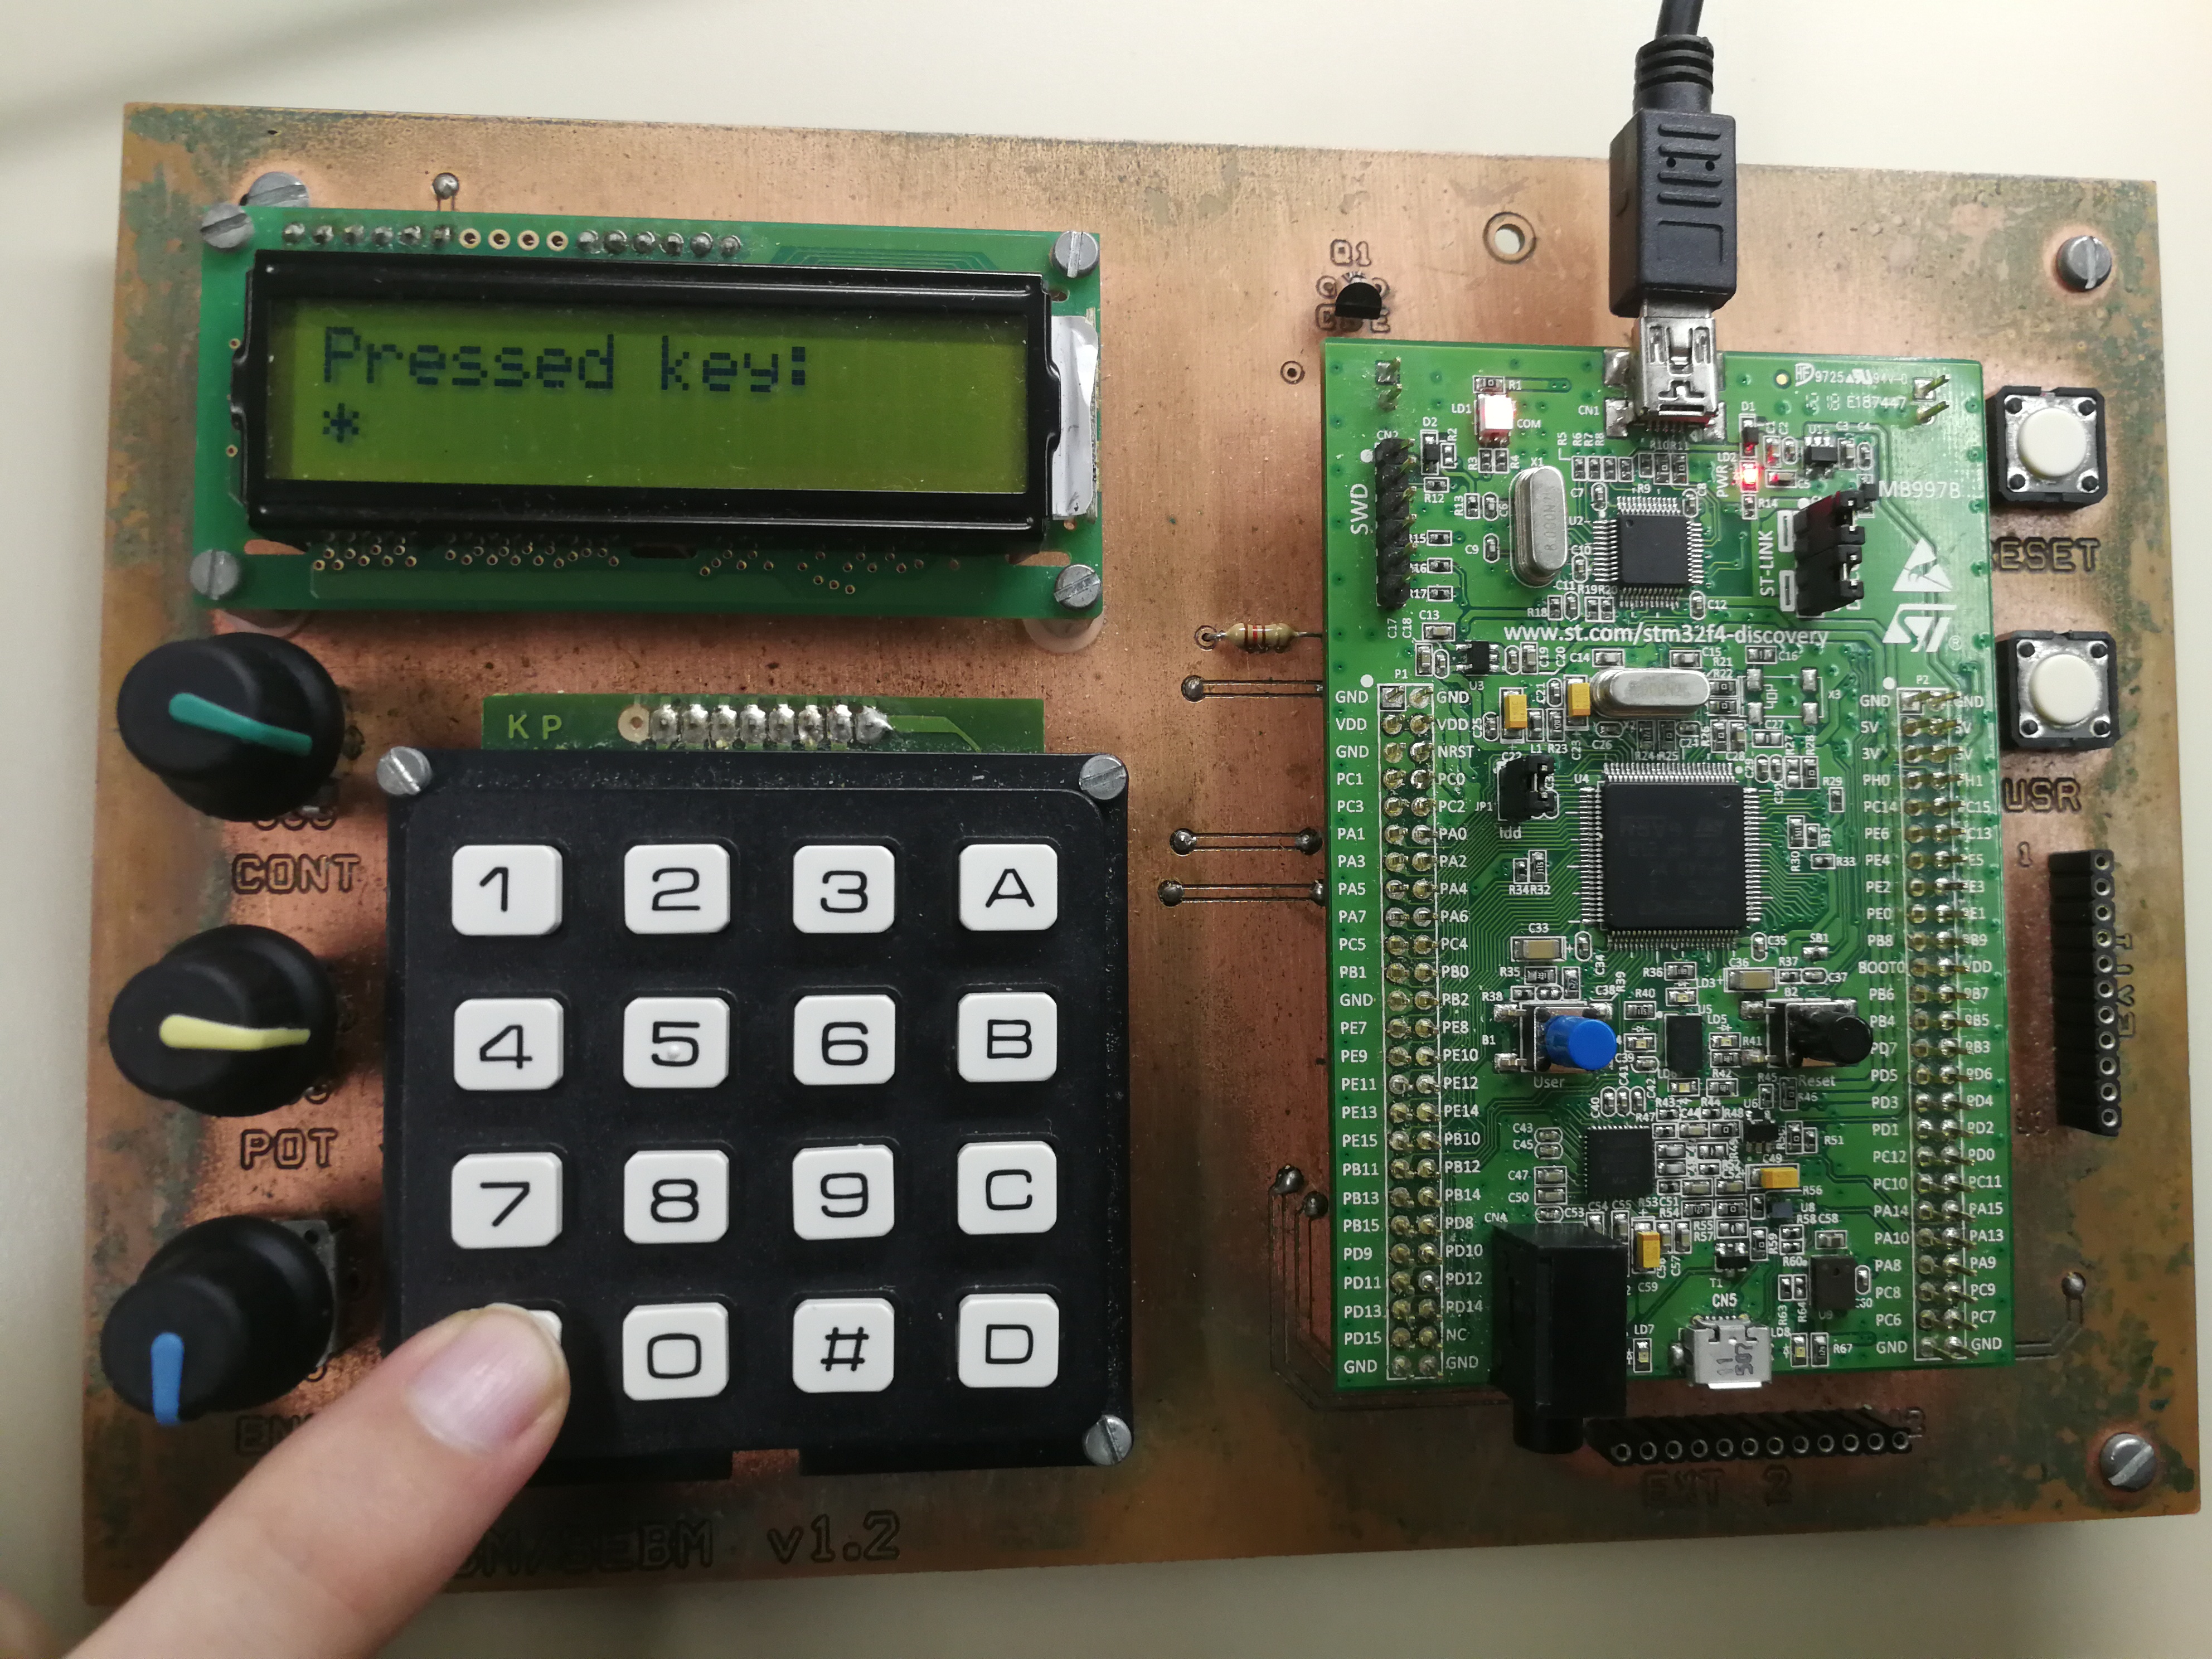
\includegraphics[width=.99\columnwidth]{../photos/board/c1-key-star}
  \caption{ \label{fig:c1-board-key-star} La placa executant la prova d'exploració del teclat, prement la tecla \texttt{*}. }
\end{figure}

\begin{figure}[p] %FIXME: subfigures?
  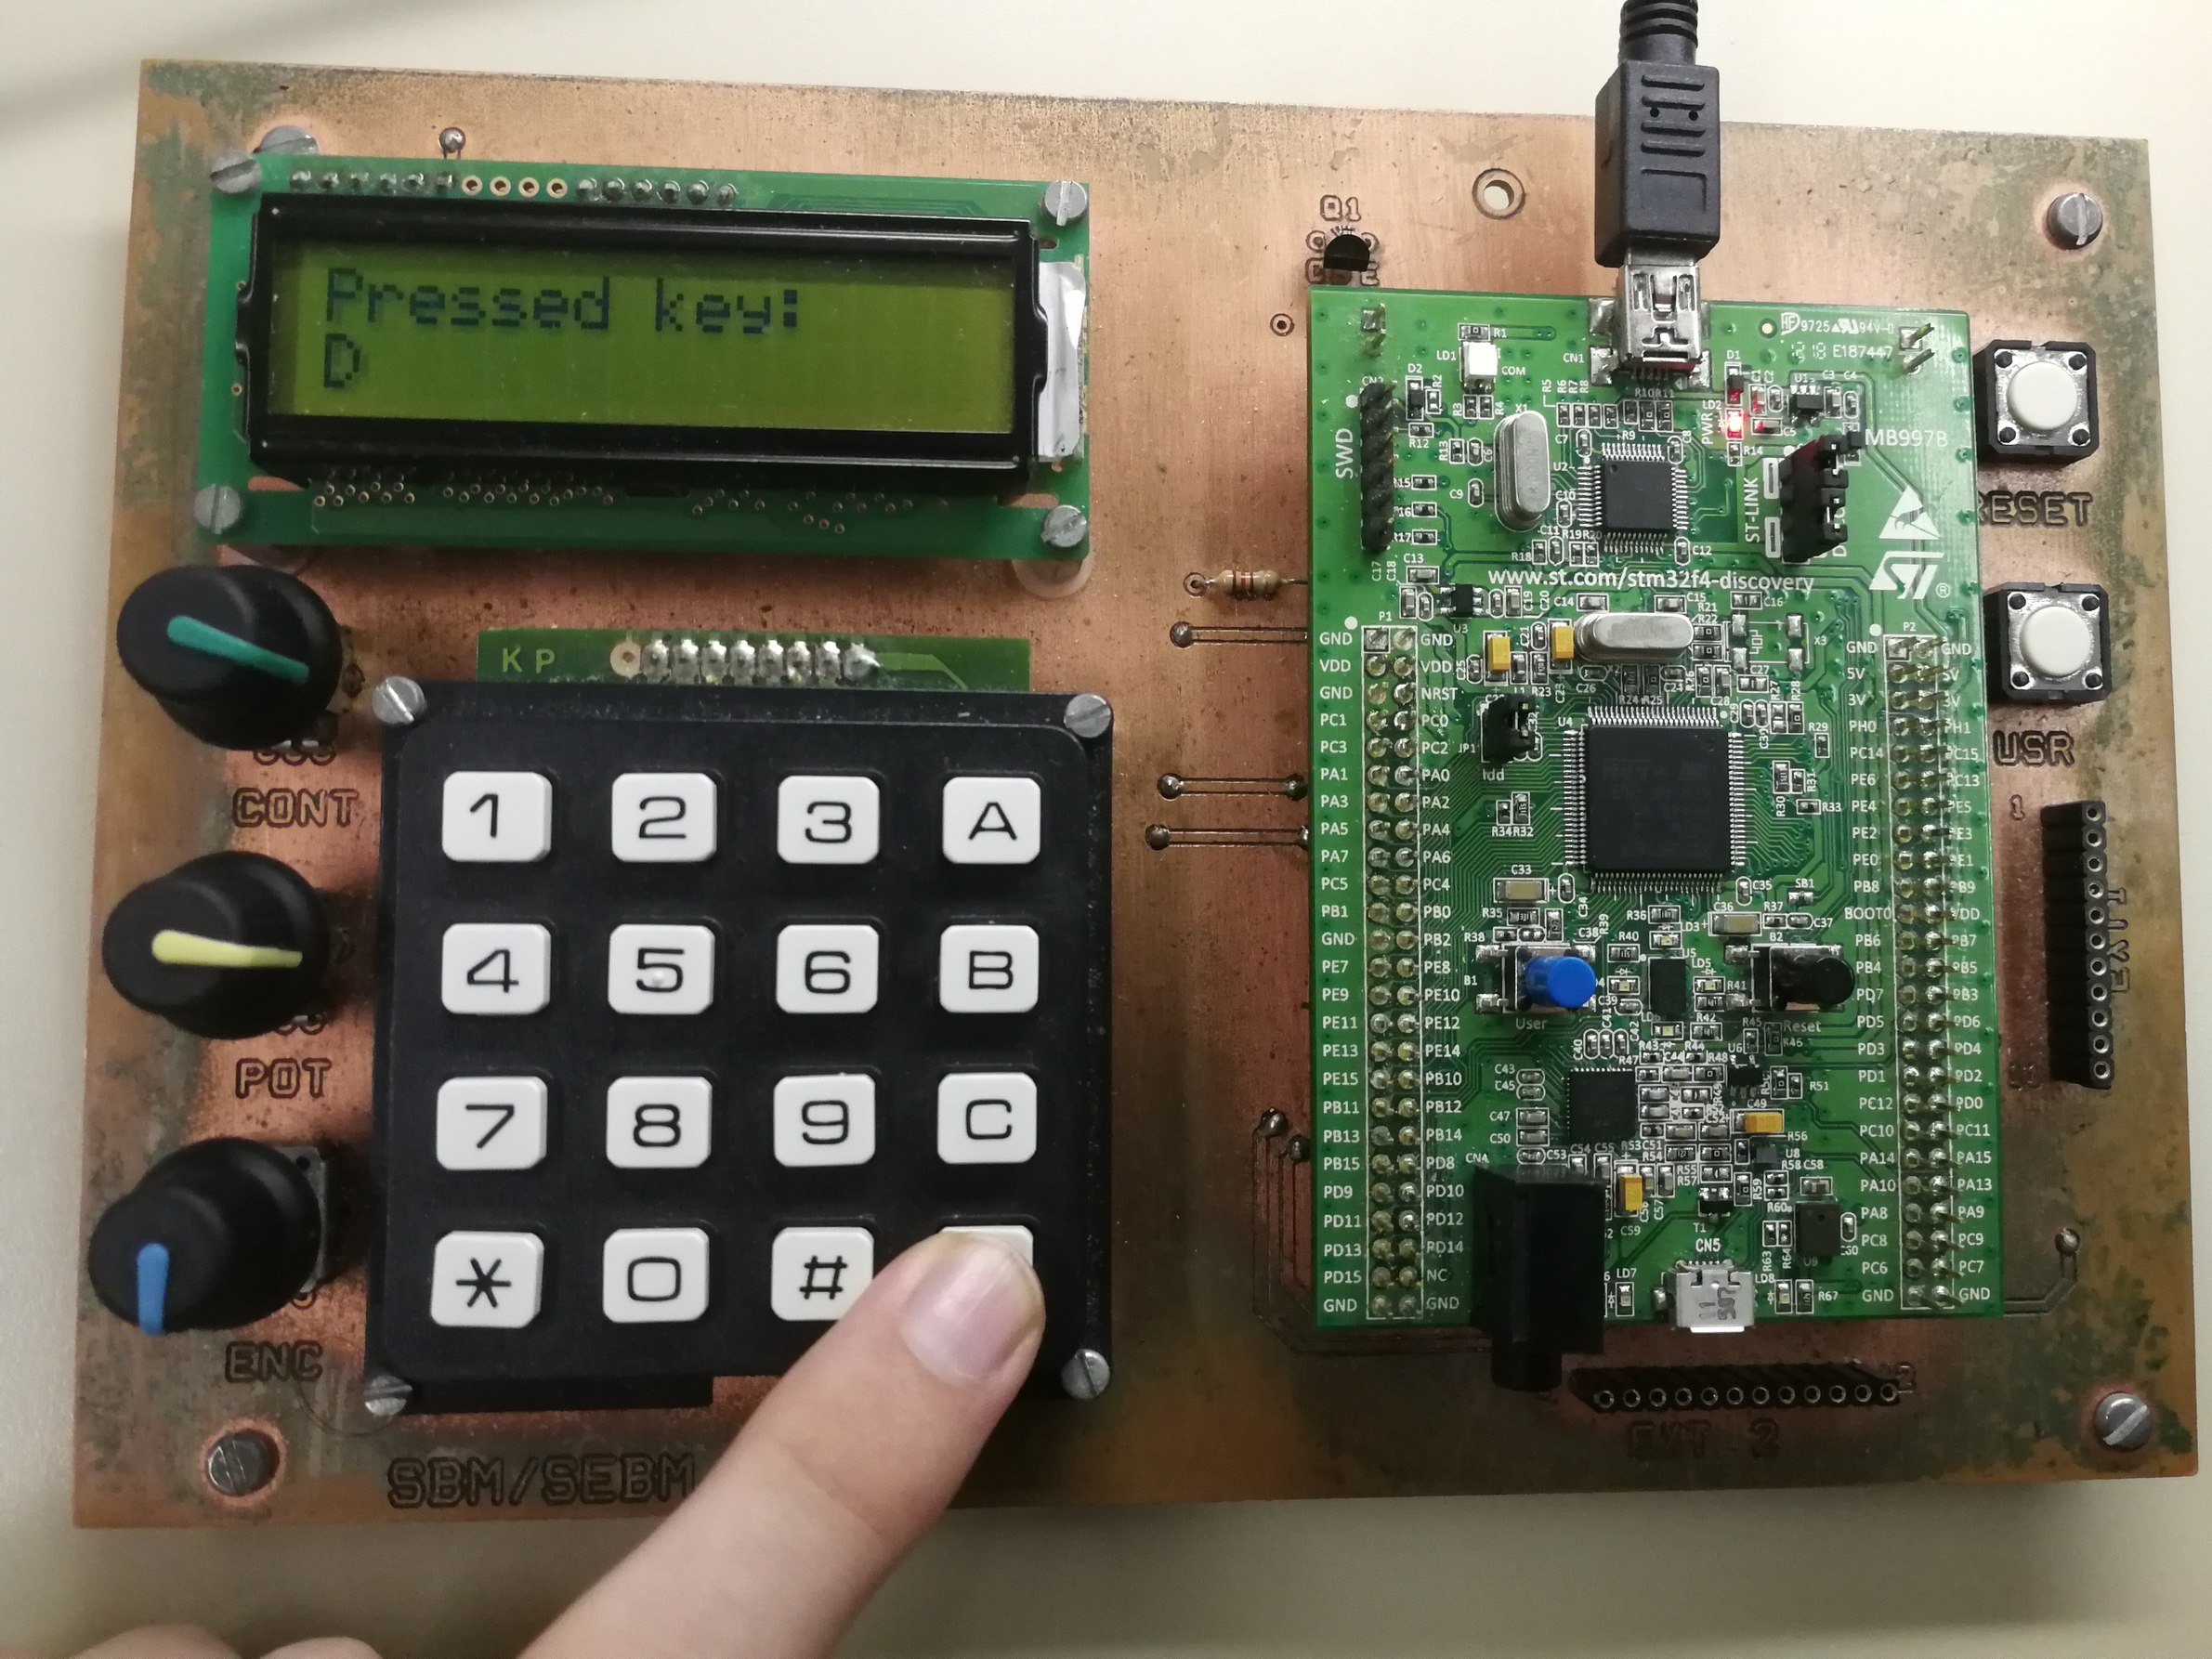
\includegraphics[width=.82\columnwidth]{../photos/board/c1-key-d}
  \caption{ \label{fig:c1-board-key-d} La placa executant la prova d'exploració del teclat, prement la tecla \texttt{D}. }
\end{figure}
\begin{figure}[p]
  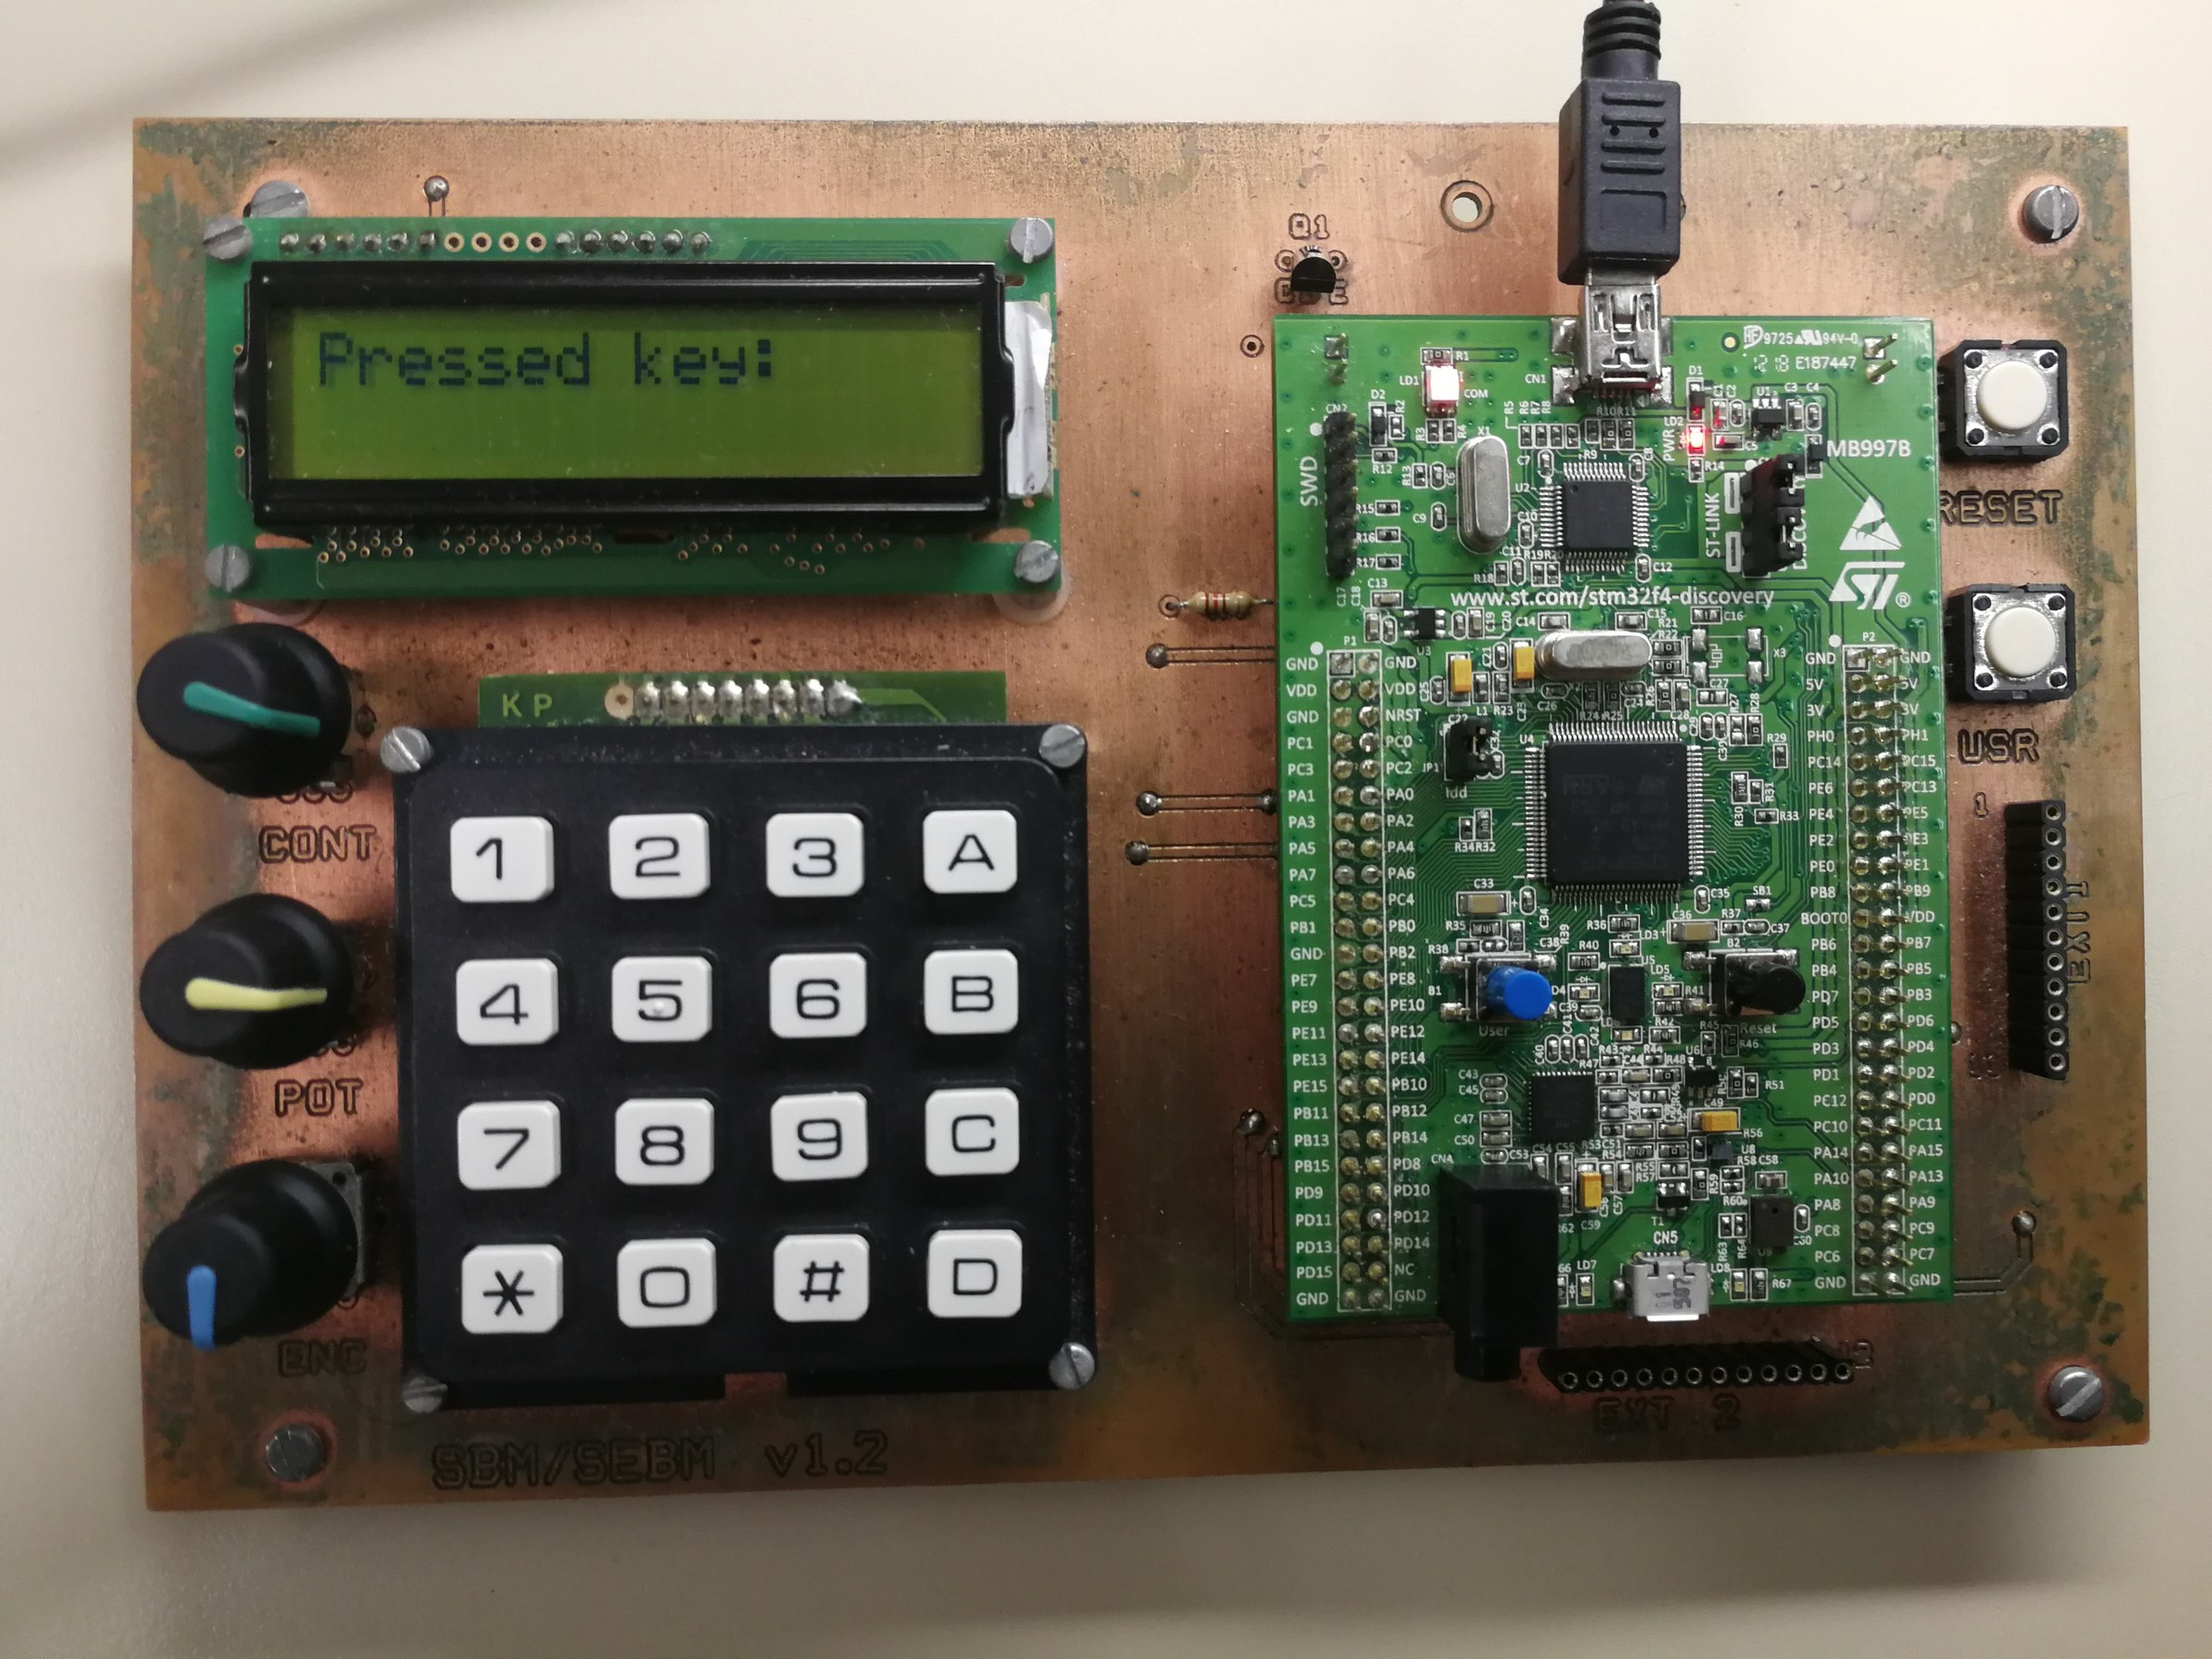
\includegraphics[width=.82\columnwidth]{../photos/board/c1-key-initial}
  \caption{ \label{fig:c1-board-key-initial} La placa executant la prova d'exploració del teclat, sense cap tecla premuda. }
\end{figure}

Tots aquests canvis a \filename{keyboard.c}, \filename{keyboard.h} i \filename{main.c}
conformen el \commit{e3974f770a876f2c8db3e061fc7d8e336201eb0e}.

\opcional
Es vol implementar una funció \fname{readMultikey} que, en comptes de retornar un únic codi de tecla
premuda, retorni una màscara de bits, amb els bits dels codis corresponents a tecles premudes habilitats.
La funció s'implementa com segueix:

\begin{minted}{c}
// Explore the full keyboard looking for any pressed keys, and return
// a 16-bit mask with bits corresponding to pressed key codes set to 1.
// Careful! Some key combinations can lead to false presses, use
// verifyPresses() to make sure no false presses are present.
int32_t readMultikey(void) {
    int32_t keys = 0;
    int32_t row;
    for (row = 0; row < 4; row++) {
        // Enable output at row
        KEY_PORT->BSRR.H.clear = BIT(KEY_ROW1_PAD + row);

        // Wait till lines are charged
        DELAY_US(8);

        // Read input pins set to 0, and set bits on keys
        int32_t cols = ((~KEY_PORT->IDR) >> KEY_COL1_PAD) & 0b1111;
        keys |= (cols << (row * 4));

        // Return row output to open
        KEY_PORT->BSRR.H.set = BIT(KEY_ROW1_PAD + row);
    }

    return keys;
}
\end{minted}
\vskip -1em

\voluntari
S'implementa també un mètode utilitat que, donat una màscara de tecles premudes,
verifica si podrien estar detectant-se falses pulsacions de tecla (que, recordem,
poden passar amb tres o més tecles premudes). La funció simplement comprova si
hi ha alguna tecla que comparteixi filera amb una segona i columna amb una tercera:

\begin{minted}{c}
// Given a pressed key mask, as returned by readMultikey(), verify
// that no incompatible key combination was found (return TRUE in that case).
int32_t verifyPresses(int32_t keys) {
    // This variable is a bit mask that accumulates the rows (bits 7..4)
    // and columns (bits 3..0) we've seen so far on pressed keys
    int32_t rowsAndCols = 0;

    // Start processing each pressed key
    int32_t key;
    for (key = 0; key < 16; key++) {
        if ((keys & BIT(key)) != 0) {
            int32_t row = key >> 2, col = key & 0b11;

            // If we've already seen both the row and the column
            // of the key, then this is an invalid combination
            if ((rowsAndCols & BIT(row + 4)) && (rowsAndCols & BIT(col)))
                return FALSE;

            // Set bits to 1, to mark row and column as seen
            rowsAndCols |= BIT(row + 4) | BIT(col);
        }
    }

    return TRUE;
}
\end{minted}
\vskip -1em

El codi s'inserta a \filename{keyboard.c} i es defineixen els prototips i la documentació
a \filename{keyboard.h}. A continuació s'escriu un programa a \filename{main.c} per mostrar
periòdicament totes les tecles premudes a l'LCD, i també avisa si la combinació podria
contenir falses pulsacions:

\begin{minted}{c}
void keyboardMultiPoll(void) {
    LCD_ClearDisplay();
    LCD_SendString("Pressed keys:");
    LCD_Config(TRUE, FALSE, FALSE);

    while (1) {
        // Wait before reading
        SLEEP_MS(100);

        // Read current keys
        int32_t keys = readMultikey();

        // Clear bottom row
        LCD_GotoXY(0, 1);
        LCD_SendString("            ");

        // Write each pressed key to LCD
        LCD_GotoXY(0, 1);
        int32_t key;
        for (key = 0; key < 16; key++) {
            if ((keys & BIT(key)) != 0)
                LCD_SendChar(KEY_CHARS[key]);
        }

        // Write error state to LCD
        LCD_GotoXY(16 - 4, 1);
        LCD_SendString(verifyPresses(keys) ? "     " : " ERR!");
    }
}
\end{minted}
\vskip -1em

Es crida des de \fname{main}, es carrega a la placa i es verifica el seu correcte
funcionament. Podem veure a la figura~\ref{fig:c1-board-keys-two} com detecta correctament
la pulsació de les tecles \texttt{7} i \texttt{*} simultàniament.

A la figura~\ref{fig:c1-board-keys-error} s'està prement \texttt{4}, \texttt{*} i \texttt{\#}
i podem veure com també es detecta la falsa pulsació de la tecla \texttt{6}, i el programa
així ho reporta.

\begin{figure}[p] %FIXME: subfigures?
  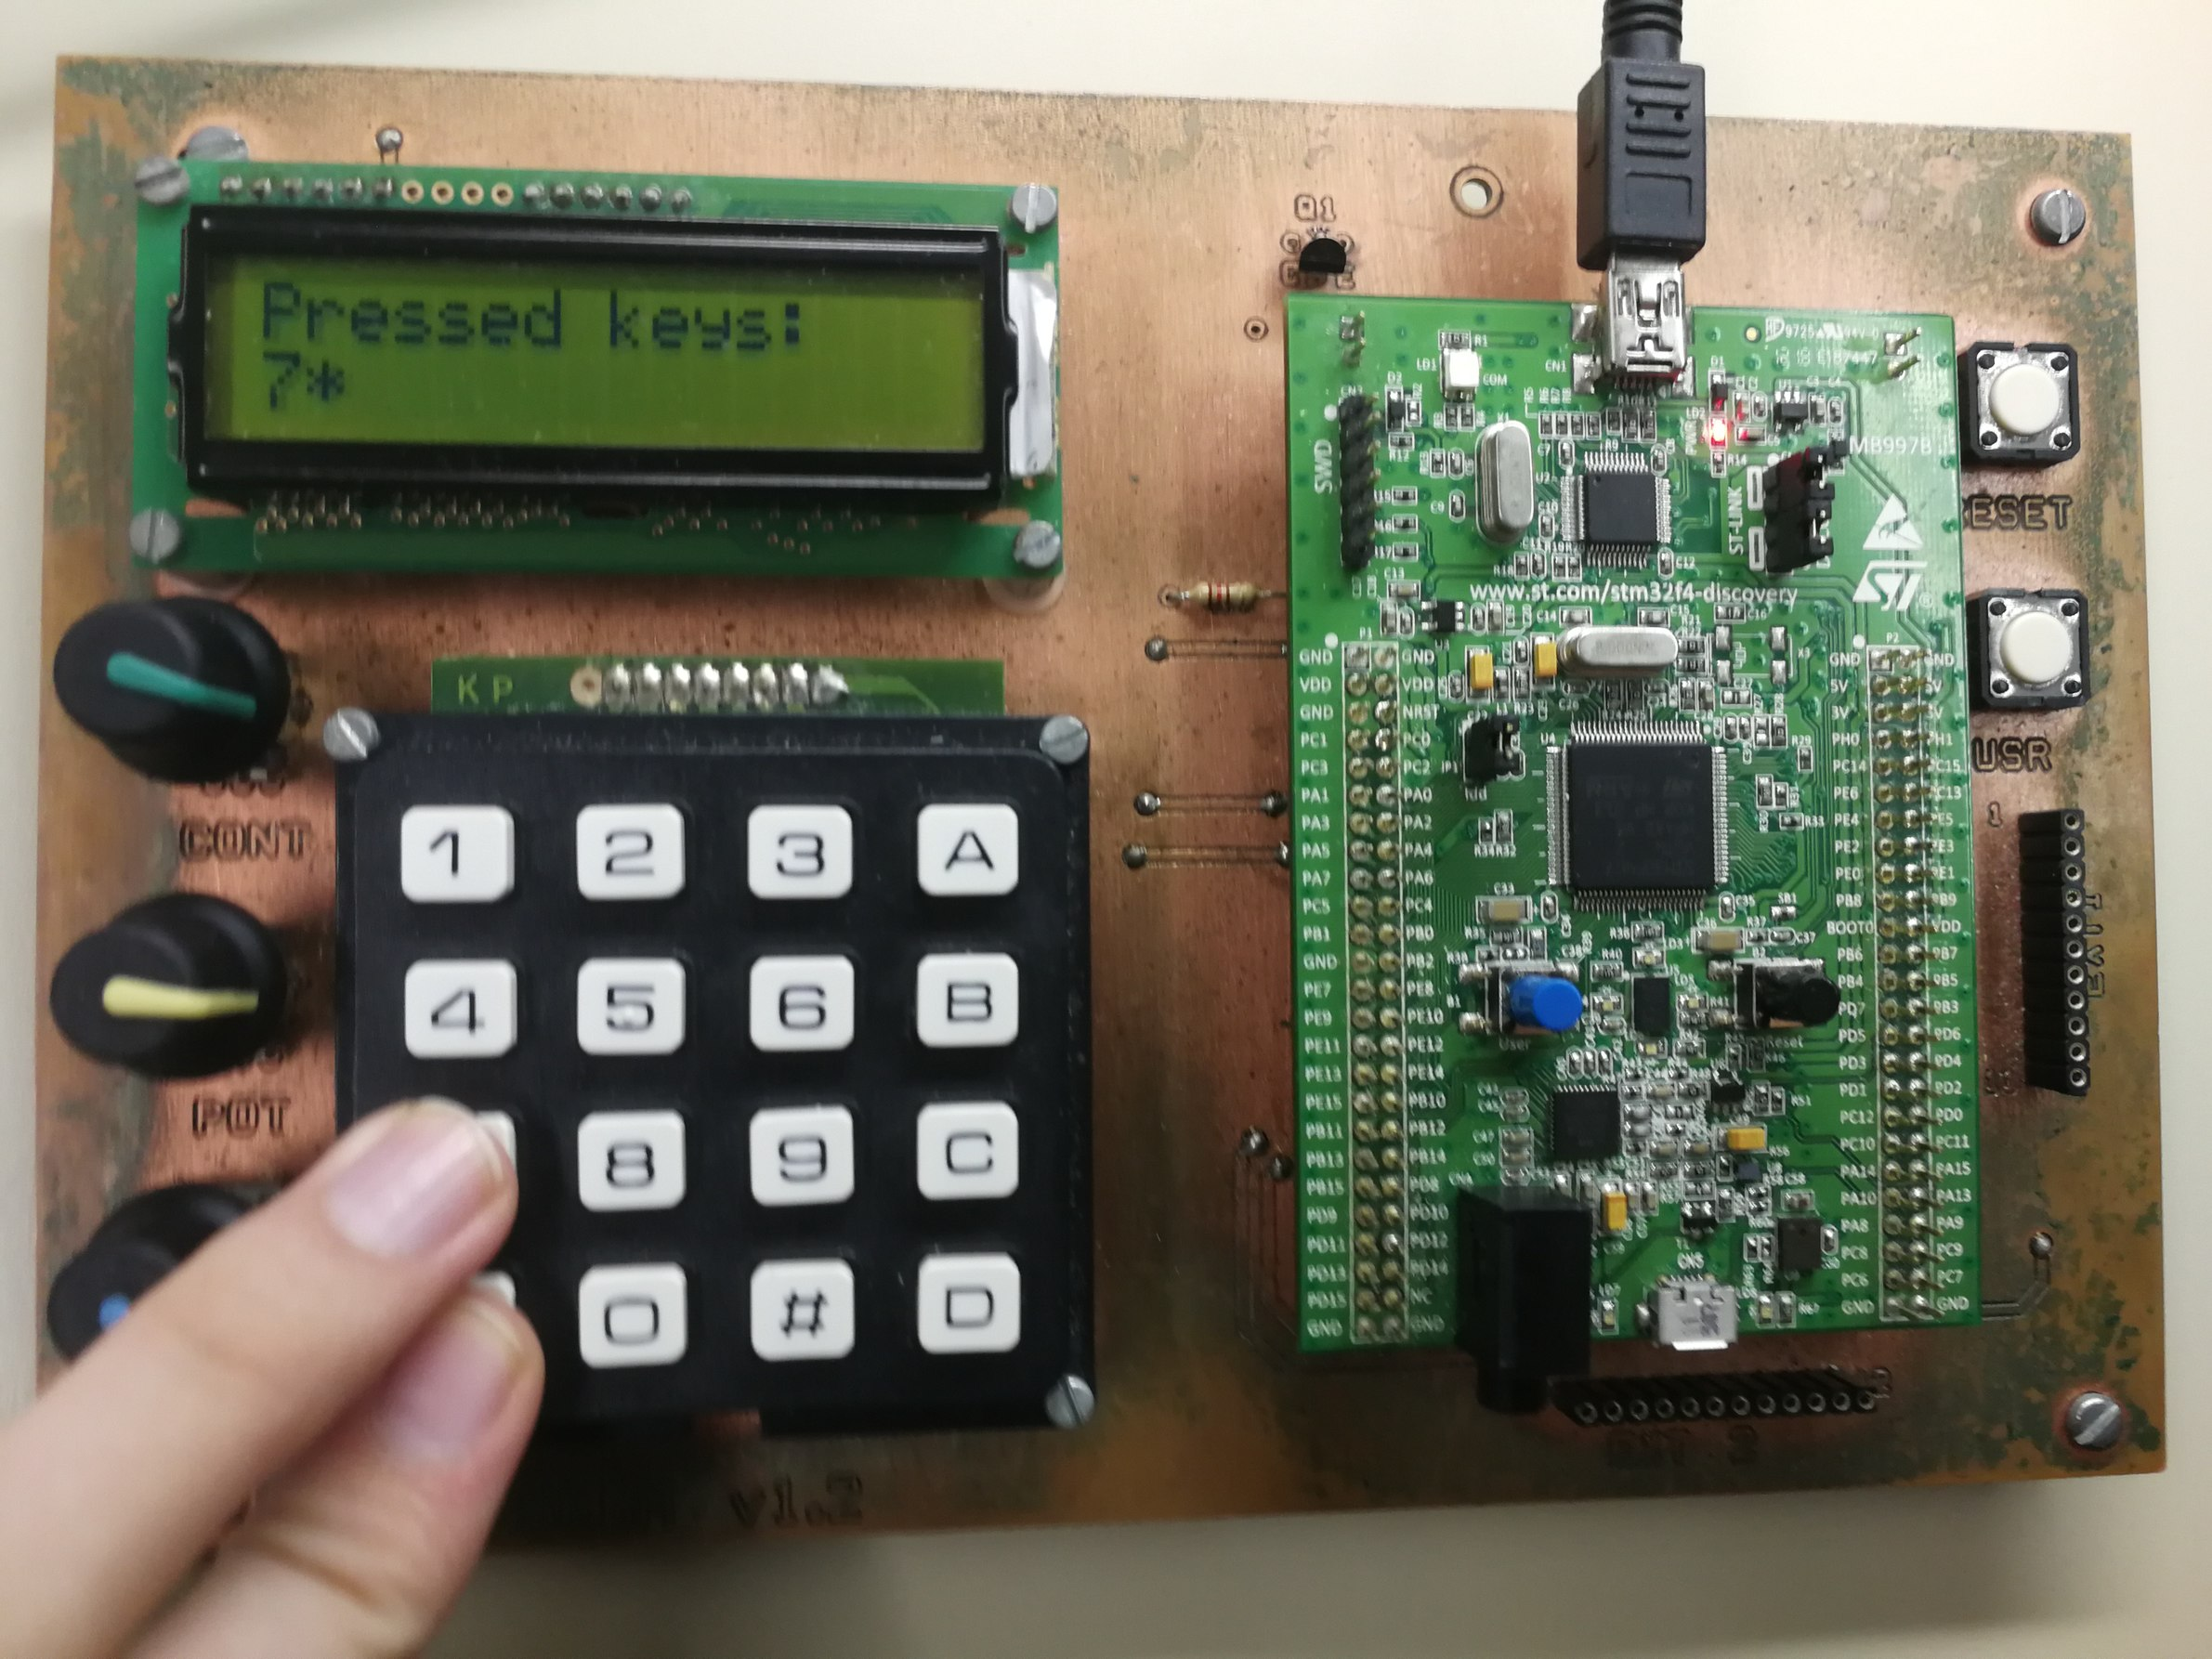
\includegraphics[width=.82\columnwidth]{../photos/board/c1-keys-two}
  \caption{ \label{fig:c1-board-keys-two} La placa detectant la pulsació simultània de les tecles \texttt{7} i \texttt{*}. }
\end{figure}
\begin{figure}[p]
  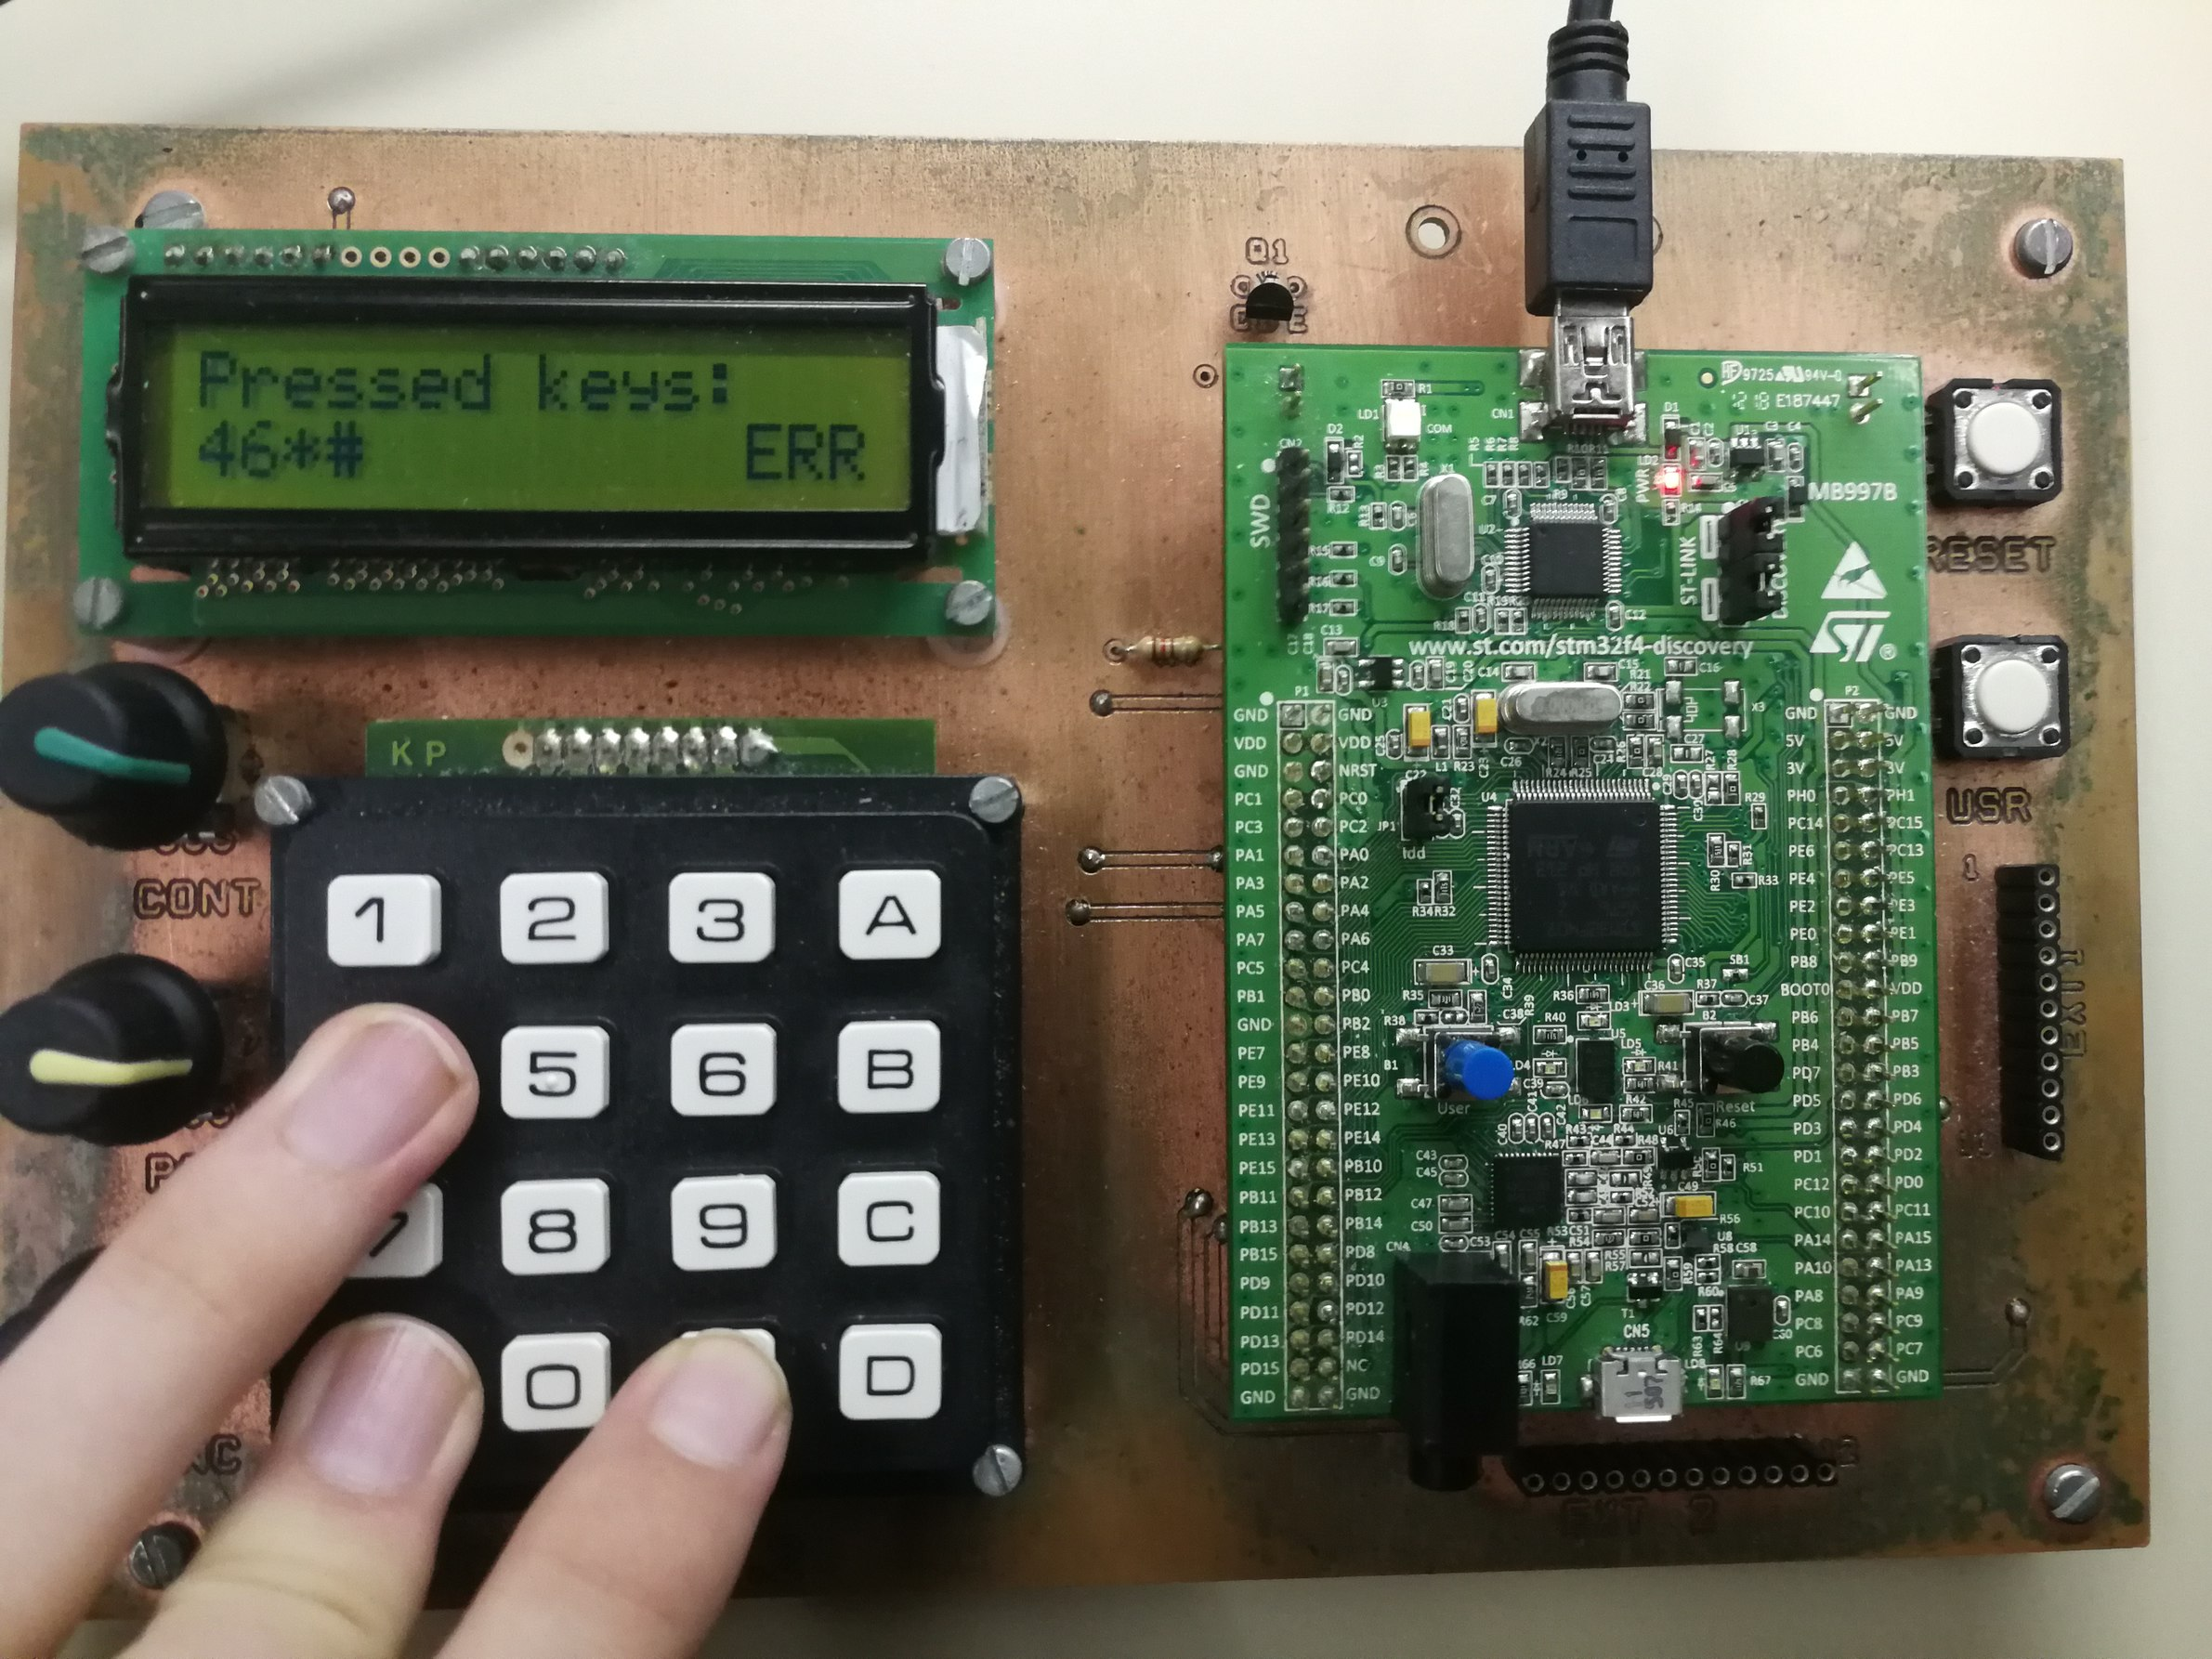
\includegraphics[width=.82\columnwidth]{../photos/board/c1-keys-error_2}
  \caption{ \label{fig:c1-board-keys-error} La placa detectant la pulsació simultània de les tecles \texttt{4}, \texttt{*} i \texttt{\#}. }
\end{figure}

Aquests canvis conformen el \commit{bfc62dd77a6e8eb1496184d78306975576243798}.

\subsection{Gestió del teclat per interrupcions}

Per últim farem la gestió del teclat mitjançant interrupcions per detectar
quan es premen tecles, en comptes de fer exploracions constants. Per fer-ho,
posem les quatre fileres a nivell baix, i activem interrupcions per flanc
de baixada en qualsevol columna.

Quan la RSI detecti una tecla al fer l'exploració, ho notificarà al programa
prinicipal desant el codi de tecla en una variable global que definim a \filename{keyboard.h}:

\begin{minted}{c}
// Global variable where last detected key is saved
extern volatile int32_t detectedKey;
\end{minted}
\vskip -1em

I que s'inicialitza a \filename{keyboard.c} al codi especial:

\begin{minted}{c}
volatile int32_t detectedKey = KEY_NOT_FOUND;
\end{minted}
\vskip -1em

Com que les línies 6 -- 9 (columnes) comparteixen vector d'interrupció,
només caldrà escriure una RSI. Aquest és el codi (estudi previ) que inicialitza
les interrupcions per flanc de baixada a les columnes i posa totes les fileres
en nivell baix (donat que no és el tema d'aquesta pràctica, no s'explica en detall):

%previ
\begin{minted}{c}
// Initialize the interrupts for key detection,
// must be called after initKeyboard()
void initConfigKeyboard(void) {
    // Put all the rows in 0 (drain) state
    KEY_PORT->BSRR.H.clear = 0b1111 << KEY_ROW1_PAD;

    // Enable SYSCFG clock and configure EXTI9..EXTI6 on the column pins
    RCC->APB2ENR |= RCC_APB2ENR_SYSCFGEN;
    SYSCFG->EXTICR[1] = (SYSCFG->EXTICR[1] & (~SYSCFG_EXTICR2_EXTI6)) | SYSCFG_EXTICR2_EXTI6_PD;
    SYSCFG->EXTICR[1] = (SYSCFG->EXTICR[1] & (~SYSCFG_EXTICR2_EXTI7)) | SYSCFG_EXTICR2_EXTI7_PD;
    SYSCFG->EXTICR[2] = (SYSCFG->EXTICR[2] & (~SYSCFG_EXTICR3_EXTI8)) | SYSCFG_EXTICR3_EXTI8_PD;
    SYSCFG->EXTICR[2] = (SYSCFG->EXTICR[2] & (~SYSCFG_EXTICR3_EXTI9)) | SYSCFG_EXTICR3_EXTI9_PD;

    // Configure falling trigger interrupts for EXTI9..EXTI6, clear pending bits
    EXTI->IMR |= EXTI_IMR_MR6 | EXTI_IMR_MR7 | EXTI_IMR_MR8 | EXTI_IMR_MR9;
    EXTI->RTSR &= ~(EXTI_RTSR_TR6 | EXTI_RTSR_TR7 | EXTI_RTSR_TR8 | EXTI_RTSR_TR9);
    EXTI->FTSR |= EXTI_FTSR_TR6 | EXTI_FTSR_TR7 | EXTI_FTSR_TR8 | EXTI_FTSR_TR9;
    EXTI->PR = EXTI_PR_PR6 | EXTI_PR_PR7 | EXTI_PR_PR8 | EXTI_PR_PR9;

    // Enable interrupt vector
    nvicEnableVector(EXTI9_5_IRQn, CORTEX_PRIORITY_MASK(STM32_EXT_EXTI5_9_IRQ_PRIORITY));
}
\end{minted}
\vskip -1em
%/previ

Després queda fer el codi de la RSI. Aquesta haurà de fer l'exploració del teclat, i si troba una
tecla desar-la a \mintinline{c}|detectedKey|. Ha de preocupar-se de desactivar les interrupcions
abans (ja que la propia exploració genera interrupcions), i al final tornar a posar les files
a nivell baix i tornar a habilitar-les. El codi resulta:

%previ
\begin{minted}{c}
// EXTI9..5 RSI associated to key presses
CH_IRQ_HANDLER(EXTI9_5_IRQHandler) {
    CH_IRQ_PROLOGUE();

    // Disable interrupts and put all rows as open
    EXTI->IMR &= ~(EXTI_IMR_MR6 | EXTI_IMR_MR7 | EXTI_IMR_MR8 | EXTI_IMR_MR9);
    KEY_PORT->BSRR.H.set = 0b1111 << KEY_ROW1_PAD;

    // Explore the keyboard and set detected key
    int32_t key = readKeyboard();
    if (key != KEY_NOT_FOUND) detectedKey = key;

    // Return rows to drain, erase pending interrupt and enable interrupts again
    KEY_PORT->BSRR.H.clear = 0b1111 << KEY_ROW1_PAD;
    EXTI->PR = EXTI_PR_PR6 | EXTI_PR_PR7 | EXTI_PR_PR8 | EXTI_PR_PR9;
    EXTI->IMR |= EXTI_IMR_MR6 | EXTI_IMR_MR7 | EXTI_IMR_MR8 | EXTI_IMR_MR9;

    CH_IRQ_EPILOGUE();
}
\end{minted}
\vskip -1em
%/previ

Llavors s'escriu un programa a \filename{main.c} que inicialitza les interrupcions
i mostra periòdicament l'última tecla detectada a l'LCD:

\begin{minted}{c}
void keyboardPollInterrupt(void) {
    // Initialize interrupts and stuff
    initConfigKeyboard();

    // Initialize LCD
    LCD_ClearDisplay();
    LCD_SendString("Pressed key:");
    LCD_Config(TRUE, FALSE, FALSE);

    // Main loop
    while (1) {
        // Wait before reading
        SLEEP_MS(100);

        // Read current key code
        int32_t key = detectedKey;

        // Write key char to LCD, or clear if no key
        LCD_GotoXY(0, 1);
        LCD_SendChar((key == KEY_NOT_FOUND) ? ' ' : KEY_CHARS[key]);
    }
}
\end{minted}
\vskip -1em

Es crida des de \fname{main}, es carrega a la placa i es comprova el correcte funcionament
d'aquest (figura~\ref{fig:c1-board-intr}). Això conforma el \commit{bb2b811708843635db03a0ef36bf905b9ca82f0e}.

\begin{figure}
  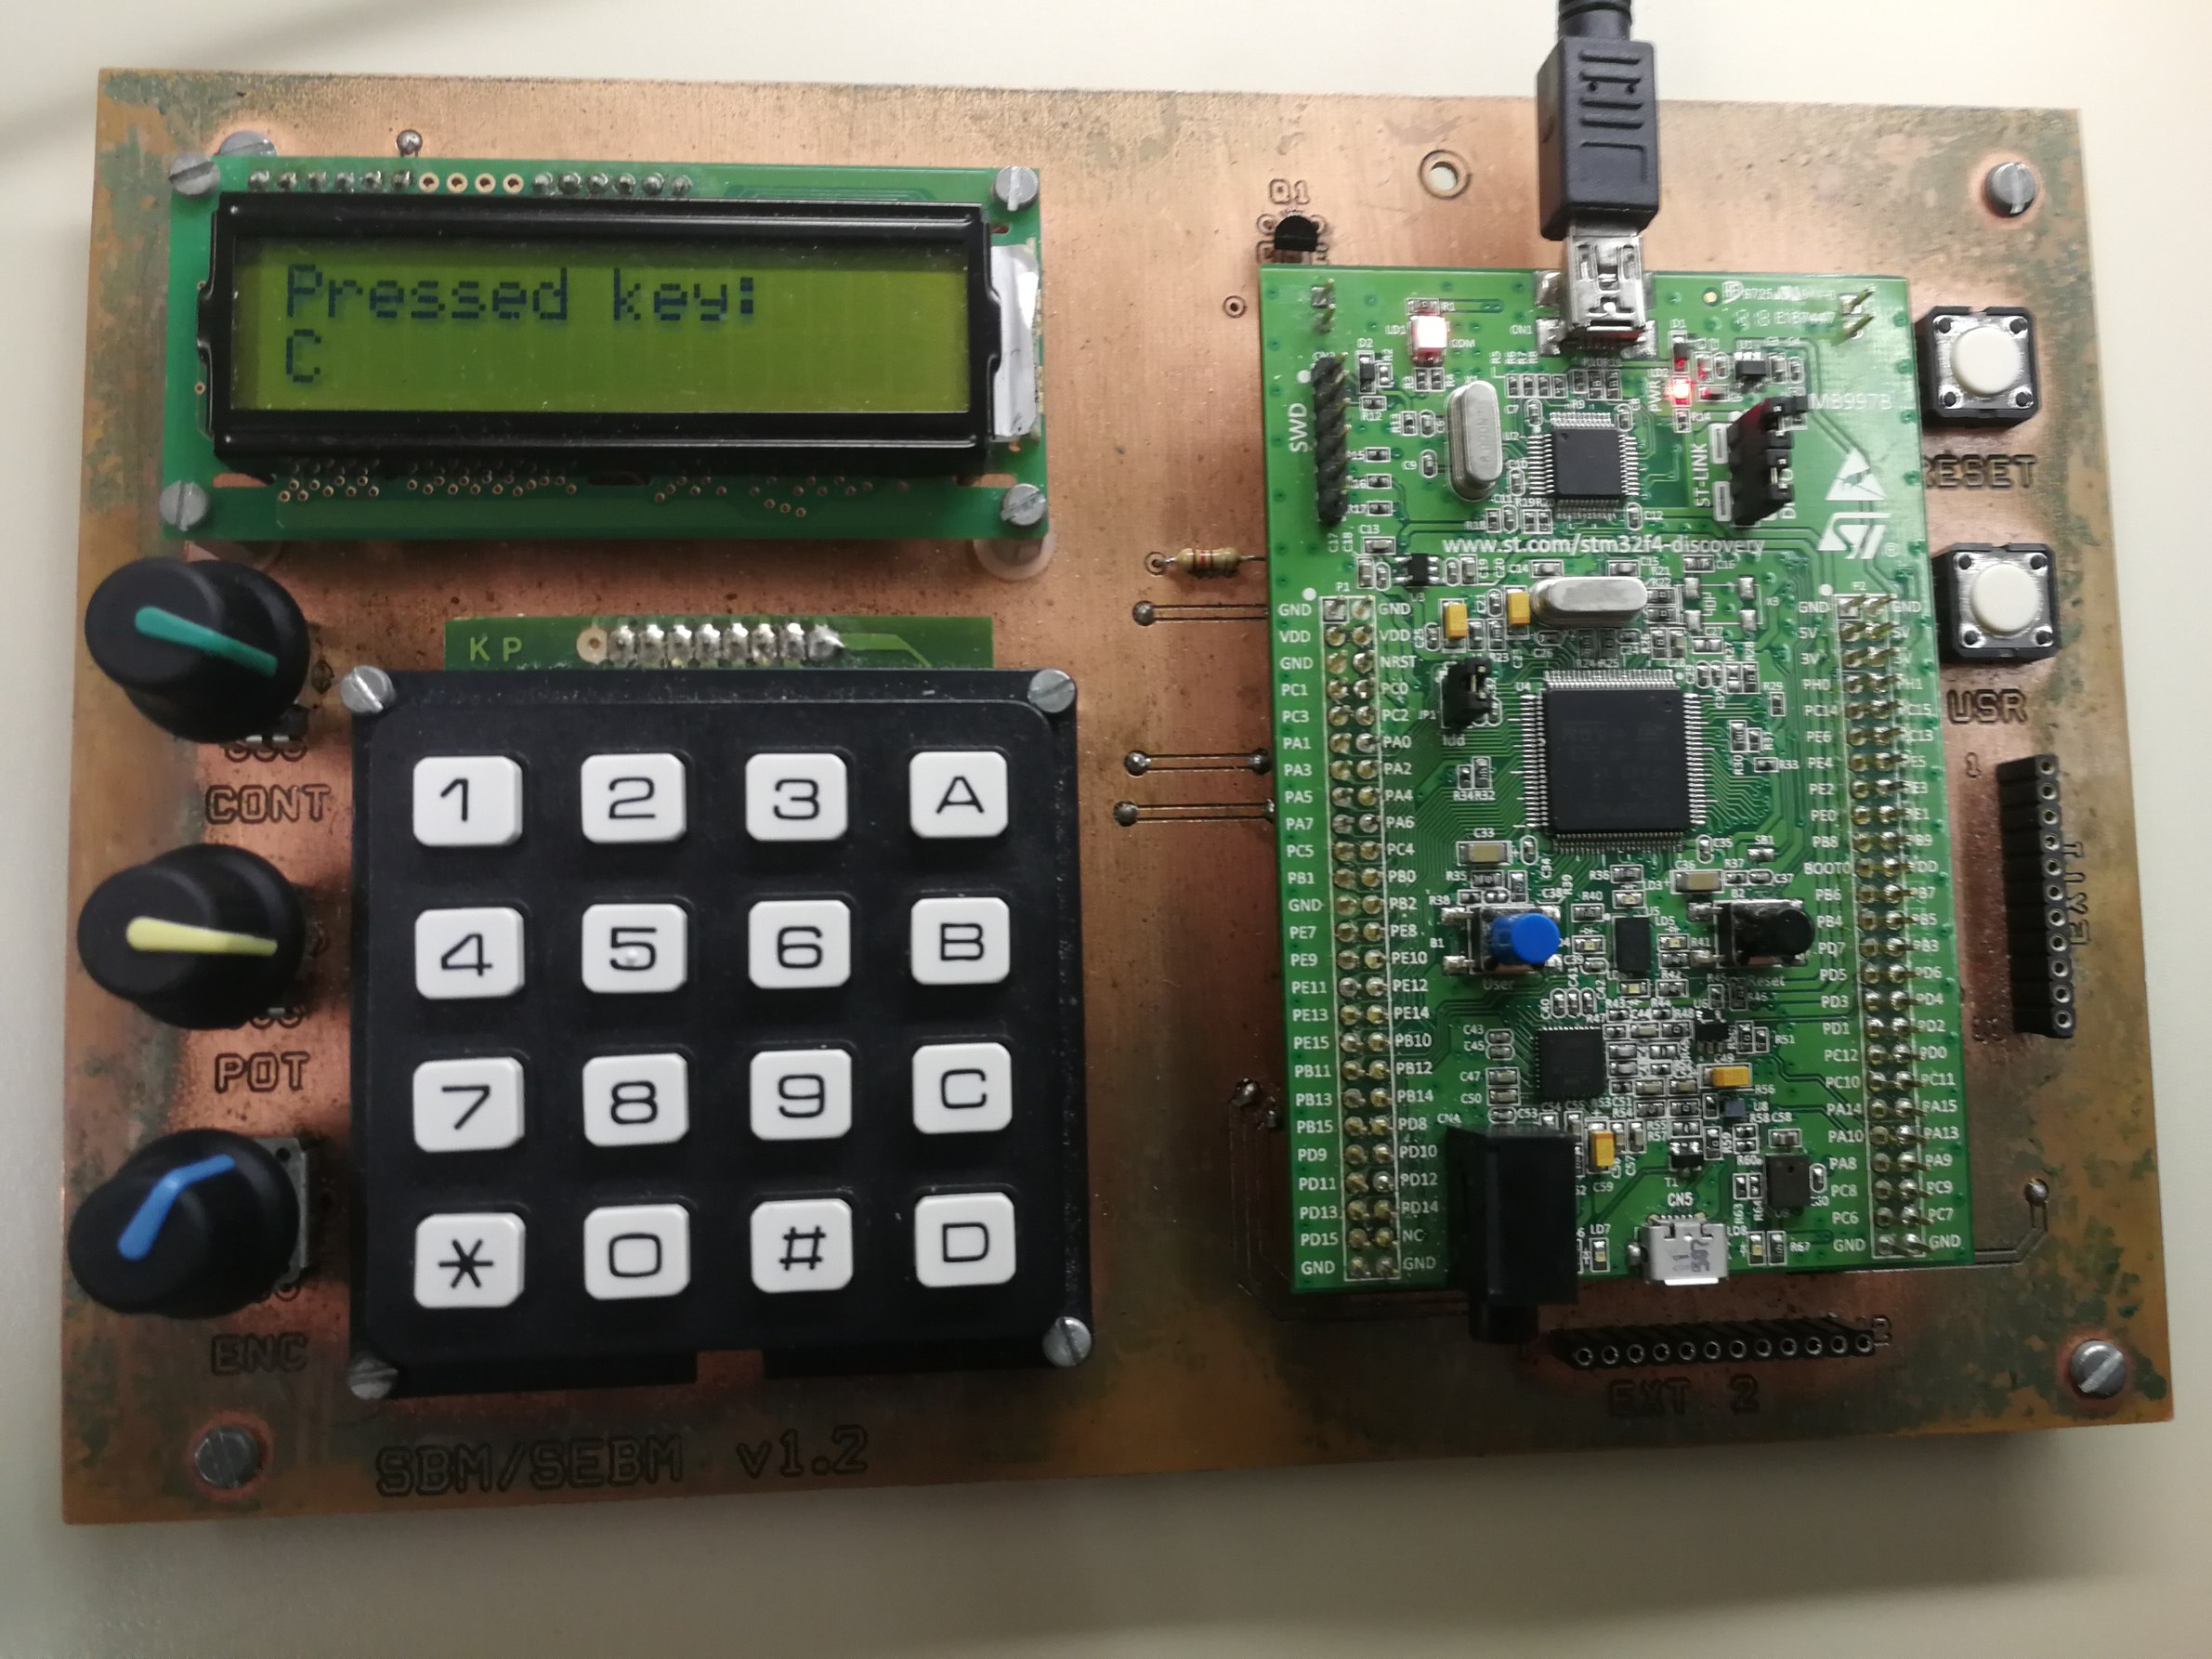
\includegraphics[width=.99\columnwidth]{../photos/board/c1-intr}
  \caption{ \label{fig:c1-board-intr} La placa executant la prova de detecció de tecles per interrupció, després de prémer \texttt{C}. }
\end{figure}


\subsection{Més propostes optatives}

S'exposen idees de programes a realitzar voluntàriament, com una calculadora o un conversor de base.
La segona ha estat realitzada, veure pàgina~\pageref{ch:basecvt}.

També s'explica el fenòmen del \emph{button bounce} o \emph{chatter} i com protegir-se contra aquest.


\section{Conclusió}

Tot i que no ha estat massa problema en aquesta pràctica, el bounce
ha estat curiós de gestionar i font de bugs especialment desenvolupant
el conversor de base. Per la resta, tot bé.

\section{Ajustaments posteriors}

Durant la realització de pràctiques posteriors s'ha vist oportú millorar la qualitat del codi de \filename{util.c}
definint una macro anomenada \fname{SET_BITS}:

\begin{minted}{c}
#define SET_BITS(value, offset, nbits, bits) \
    value = ((value) & ~((BIT(nbits)-1) << (offset))) | ((bits) << (offset));
\end{minted}
\vskip -1em

Que manipula una quantitat de bits \mintinline{c}|nbits| començant pel bit més baix \mintinline{c}|offset|,
establint aquests bits al valor de \mintinline{c}|bits|. Amb això, el codi de \fname{GPIO_ModeInput} i
\fname{GPIO_ModePushPull} esdevé:

\begin{minted}{c}
/* ... */
void GPIO_ModeOpenDrain(GPIO_TypeDef *port, int32_t line) {
    line &= 0xF;

    // OTy -> 1 Open drain output
    SET_BITS(port->OTYPER, line, 1, 1);

    // OSPEEDRy[1:0] -> 00 Speed 25MHz
    SET_BITS(port->OSPEEDR, 2*line, 2, 0b00);

    // PUPDRy[1:0] -> 00 No pull-up, no pull-down
    SET_BITS(port->PUPDR, 2*line, 2, 0b00);

    // ODRy -> 1 Open
    SET_BITS(port->ODR, line, 1, 1);

    // After everything is set up, switch mode
    // MODERy[1:0] -> 01 General purpose output mode
    SET_BITS(port->MODER, 2*line, 2, 0b01);
}

/* ... */
void GPIO_ModeInput(GPIO_TypeDef *port, int32_t line, int32_t pullUpDown) {
    line &= 0xF;

    // MODERy[1:0] -> 00 Input
    SET_BITS(port->MODER, 2*line, 2, 0b00);

    // PUPDRy[1:0] -> [as requested]
    SET_BITS(port->PUPDR, 2*line, 2, pullUpDown & 0b11);

    // ODRy -> 1
    SET_BITS(port->ODR, line, 1, 1);
}
\end{minted}
\vskip -1em

També s'afegeix l'ordre \mintinline{c}|line &= 0xF;| al principi, que assegura que \mintinline{c}|line|
estigui entre 0 i 15 (per seguretat). Tot això és el \commit{da6142aab1f1cf2a6bafaa3d98a55262c5f985bb}.

Més endavant al \commit{d6babe86f524c875e7b5d9e93cf336c434c1b18c} també es corregeix (junt
amb el bug de l'LCD) l'ordre en que es manipulen els registres, de forma que MODER es
configuri al final, quan ODR i la resta ja tenen els valors correctes. Així, si el port
estava en mode entrada, no deixarà mai d'estar en alta impedància quan el passem a
sortida en drenador obert:

\begin{minted}{diff}
--- a/util.c
+++ b/util.c
@@ -42,9 +43,6 @@ void GPIO_ModePushPull(GPIO_TypeDef *port, int32_t line) {
 void GPIO_ModeOpenDrain(GPIO_TypeDef *port, int32_t line) {
     line &= 0xF;
 
-    // MODERy[1:0] -> 01 General purpose output mode
-    SET_BITS(port->MODER, 2*line, 2, 0b01);
-
     // OTy -> 1 Open drain output
     SET_BITS(port->OTYPER, line, 1, 1);
 
@@ -56,6 +54,10 @@ void GPIO_ModeOpenDrain(GPIO_TypeDef *port, int32_t line) {
 
     // ODRy -> 1 Open
     SET_BITS(port->ODR, line, 1, 1);
+
+    // After everything is set up, switch mode
+    // MODERy[1:0] -> 01 General purpose output mode
+    SET_BITS(port->MODER, 2*line, 2, 0b01);
 }
 
 // Configure a GPIO line as input
\end{minted}
\vskip -1em

Finalment, en el \commit{00ea9a601daa4bbfe8685a5a59c29e3aea24478f} s'ha mogut la funció
\fname{itoa}, que es dona ja feta, al fitxer \filename{util.c} i s'ha definit al header
corresponent. Així la podem fer servir des d'altres mòduls o programes.
